\documentclass{ctexart}
\PassOptionsToPackage{numbers,compress}{natbib}
% Common packages
\usepackage[utf8]{inputenc} % allow utf-8 input
\usepackage[T1]{fontenc}    % use 8-bit T1 fonts
\usepackage{microtype}
\usepackage{times}
\usepackage{graphicx}
\usepackage{amsmath,amssymb,mathbbol}
% \usepackage{algorithmic}
% \usepackage[linesnumbered,ruled,vlined]{algorithm2e}
\usepackage{acronym}
\usepackage{enumitem}
\usepackage[pagebackref=true,breaklinks=true,colorlinks]{hyperref}
\usepackage{balance}
\usepackage{xspace}
\usepackage{setspace}
\usepackage[skip=3pt,font=small]{subcaption}
\usepackage[skip=3pt,font=small]{caption}
\usepackage[dvipsnames]{xcolor}
\usepackage[capitalise]{cleveref}
\usepackage{booktabs,tabularx,colortbl,multirow,array,makecell}
\usepackage{indentfirst} 
% \usepackage{overpic,wrapfig}

\usepackage{fancyhdr}
\hypersetup{pdfencoding=auto,colorlinks=true,allcolors=black}
\renewcommand{\headrulewidth}{0.5pt}
\renewcommand{\footrulewidth}{0pt}
\fancyhf{}
\fancyhead[C]{}
\fancyhead[C]{}
\fancyfoot[C]{\thepage}

% Handy shorthand
\makeatletter
\DeclareRobustCommand\onedot{\futurelet\@let@token\@onedot}
\def\@onedot{\ifx\@let@token.\else.\null\fi\xspace}
\def\eg{\emph{e.g}\onedot} 
\def\Eg{\emph{E.g}\onedot}
\def\ie{\emph{i.e}\onedot} 
\def\Ie{\emph{I.e}\onedot}
\def\cf{\emph{c.f}\onedot} 
\def\Cf{\emph{C.f}\onedot}
\def\etc{\emph{etc}\onedot} 
\def\vs{\emph{vs}\onedot}
\def\wrt{w.r.t\onedot} 
\def\dof{d.o.f\onedot}
\def\etal{\emph{et al}\onedot}
\makeatother

\definecolor{gray}{gray}{0.9}

% Handy math ops
\DeclareMathOperator*{\argmax}{arg\,max}
\DeclareMathOperator*{\argmin}{arg\,min}
\newcommand{\norm}[1]{\left\Vert #1 \right\Vert}

% % Spacing
\frenchspacing
% \medmuskip=2mu   % reduce spacing around binary operators
% \thickmuskip=3mu % reduce spacing around relational operators
% \setlength{\abovedisplayskip}{3pt}
% \setlength{\belowdisplayskip}{3pt}
% \setlength{\abovecaptionskip}{3pt}
% \setlength{\belowcaptionskip}{3pt}
\setlength\floatsep{0.5\baselineskip plus 3pt minus 2pt}
\setlength\textfloatsep{0.5\baselineskip plus 3pt minus 2pt}
\setlength\dbltextfloatsep{0.5\baselineskip plus 3pt minus 2pt}
\setlength\intextsep{0.5\baselineskip plus 3pt minus 2pt}

\makeatletter
\renewcommand{\paragraph}{%
  \@startsection{paragraph}{4}%
  {\z@}{0ex \@plus 0ex \@minus 0ex}{-1em}%
  {\hskip\parindent\normalfont\normalsize\bfseries}%
}
\makeatother

% Graphics path
\graphicspath{{figures/}}

% Clever references
\crefname{algorithm}{Alg.}{Algs.}
\Crefname{algorithm}{Algorithm}{Algorithms}
\crefname{section}{Sec.}{Secs.}
\Crefname{section}{Section}{Sections}
\crefname{table}{Tab.}{Tabs.}
\Crefname{table}{Table}{Tables}
\crefname{figure}{Fig.}{Fig.}
\Crefname{figure}{Figure}{Figure}

% Acronym
\acrodef{pku}[PKU]{Peking University}
\usepackage[final]{template22}
\setlength{\parindent}{2em}

\title{Lab1-MarchingCube}
\author{王想 2100013146}
\date{}
\begin{document}
\maketitle

\section{算法实现}
\subsection{对立方体顶点和边的顺序约定}
为了便于用for循环统一处理边与顶点,规定每个网格顶点和边的顺序如下:
\begin{figure}[htbp]
    \centering
    
\includegraphics[width=0.5\linewidth]{figures/order.png}
    \caption{\textbf{Order}}
\end{figure}

在这样的规定下,可以通过位运算得到每个顶点的位置和每条边的起止点。
假设立方体 $v_0$ 顶点的位置为 $v_0 = (x, y, z)$,则第 $i$ 个顶点 $v_i$ 的位置为
$$v_i = (x + \text{i \& 1}, y + \text{i >> 1 \& 1}, z + \text{i >> 2 \& 1})$$
第 $j$ 条边$e_j$的起始点为
$$v_0 + (\text{j \& 1}) \cdot unit(\text{((j >> 2) + 1) \% 3}) + (\text{j >> 1 \& 1}) unit(\text{((j >> 2) + 2) \% 3})$$
其方向为
$unit(\text{j >> 2})$,
其中 $unit(k)$ 表示第k个方向的单位向量,
$unit(0) = (1, 0, 0)$,$unit(1) = (0, 1, 0)$,$unit(2) = (0, 0, 1)$。
并且,这个顺序与表中的顺序对应,比如查询EdgeStateTable时,
$edges = EdgeStateTable[index]$中edges的第 i 位记录了第 i 条边的信息,
(为1表示第i条边上有顶点)。



\subsection{算法步骤}
有了上述的规定后,
我们可以直接用for循环遍历每一个小立方体的8个顶点和12条边。
对每一个小正方体,首先遍历8个顶点并查询该点处的SDF函数值,
获取对应这个小立方体在表中的立方体索引值$index$。

然后根据立方体索引$index$在表$EdgeStateTable$中查询边的状态,
利用查询到的边的状态遍历12条边并用
$record_{1\times12}$记录对应边上的顶点在网格顶点集中的索引。
若边$e_j$上不存在网格顶点则$record[j]=-1$。
如果边$e_j$上存在网格顶点,
为了防止网格的顶点集中顶点的重复,
必须先在网格的顶点集中查询该顶点是否存在,
如果顶点集中已经存在,则$record[j]$直接存入在网格的顶点集中查询到的该顶点对应的索引;
如果顶点集中不存在,则将该顶点加入网格的顶点集,$record[j]$存入该顶点的索引。

最后,根据立方体索引$index$在表$EdgeOrdsTable$中查询三角面的顶点连接方式,
按照查询到的连接方式将$record$记录的顶点索引加入网格的三角面片集中。

在上述操作过程中会计算网格顶点坐标和网格顶点法向并存入顶点集与法向集,
网格顶点坐标的计算是根据边的两个端点处的SDF值进行线性插值,
找到SDF=0的位置作为该网格顶点的坐标。
网格顶点法向的计算则是根据边的两个端点处的SDF的梯度值并利用上面计算出的比例

\subsection{特殊处理}
考虑到对于某些SDF数据,
可能会有立方体边上的网格顶点极其靠近边的顶点,
导致最后超出float32类型计算的精度,
使得最后计算出的该网格顶点的坐标等于边的顶点的坐标,
进而导致某些三角面的三个顶点的索引值相同。
以图1为例,如果边$e_0,e_4,e_8$上均存在网格顶点且均趋近于点$v_0$,
超出计算精度后计算得到这三个点坐标均为$v_0$的坐标,
此时这三个点组成的面会被记录成有三个$v_0$组成的面。

为了应对这种情况,我对网格顶点与立方体顶点的距离进行限制,
若立方体顶点处SDF值为0,网格顶点位于立方体顶点处,
否则,网格顶点离立方体顶点的距离不得小于$10^{-5}$。
在这个限制下可以有效避免上述问题,并且不影响网格的生成效果。

进行线性插值得到。



\section{Results}
\begin{figure}[htbp]
    \centering
    \begin{subfigure}[htbp]{0.3\linewidth}
        \centering
        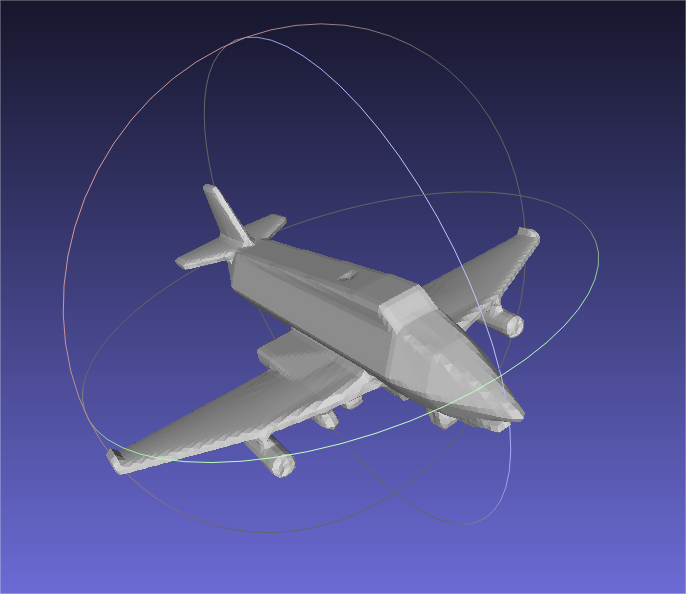
\includegraphics[width=0.9\linewidth]{figures/1_1.png}
        \caption{\textbf{01.sdf}}
    \end{subfigure}
    \begin{subfigure}[htbp]{0.3\linewidth}
        \centering
        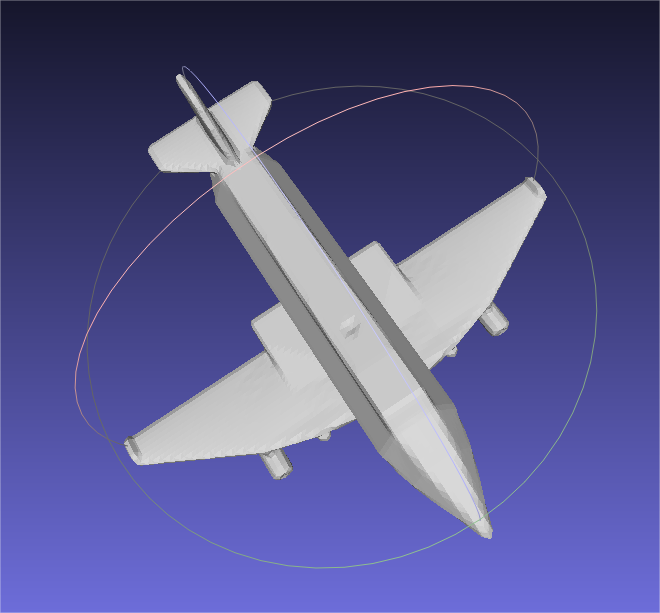
\includegraphics[width=0.9\linewidth]{figures/1_2.png}
        \caption{\textbf{01.sdf}}
    \end{subfigure}
    \begin{subfigure}[htbp]{0.3\linewidth}
        \centering
        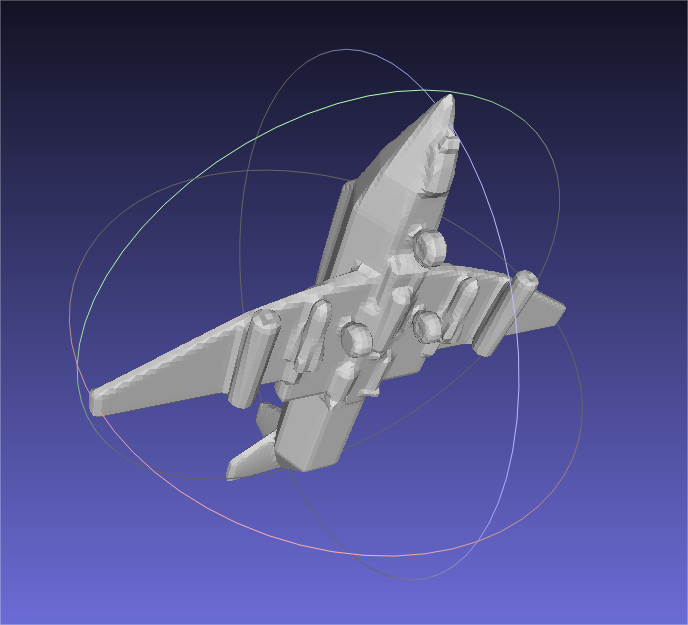
\includegraphics[width=0.9\linewidth]{figures/1_3.png}
        \caption{\textbf{01.sdf}}
    \end{subfigure}
    \begin{subfigure}[htbp]{0.3\linewidth}
        \centering
        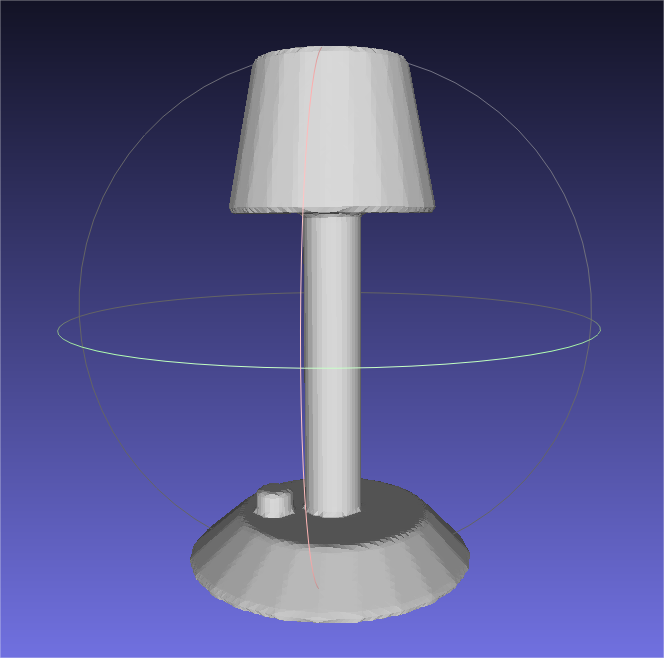
\includegraphics[width=0.9\linewidth]{figures/2_1.png}
        \caption{\textbf{02.sdf}}
    \end{subfigure}
    \begin{subfigure}[htbp]{0.3\linewidth}
        \centering
        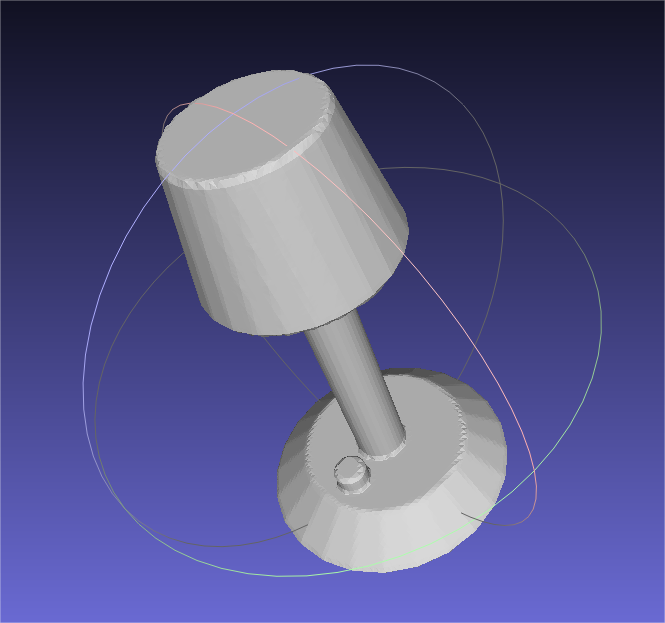
\includegraphics[width=0.9\linewidth]{figures/2_2.png}
        \caption{\textbf{02.sdf}}
    \end{subfigure}
    \begin{subfigure}[htbp]{0.3\linewidth}
        \centering
        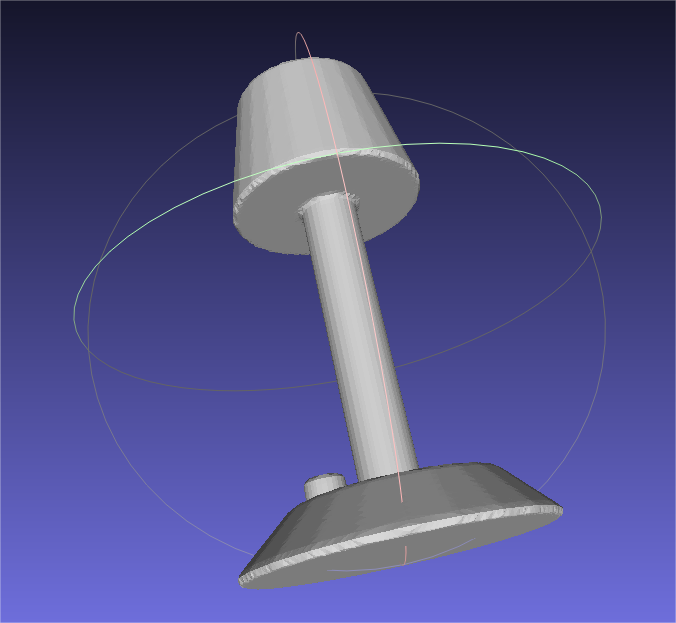
\includegraphics[width=0.9\linewidth]{figures/2_3.png}
        \caption{\textbf{02.sdf}}
    \end{subfigure}
    \caption{\textbf{Mesh}}
\end{figure}

\appendix
\section{Appendix}
Requirement: $numpy$

Running command: $python\ main.py$


\end{document}